\documentclass{standalone}
\usepackage{tikz}

\begin{document}

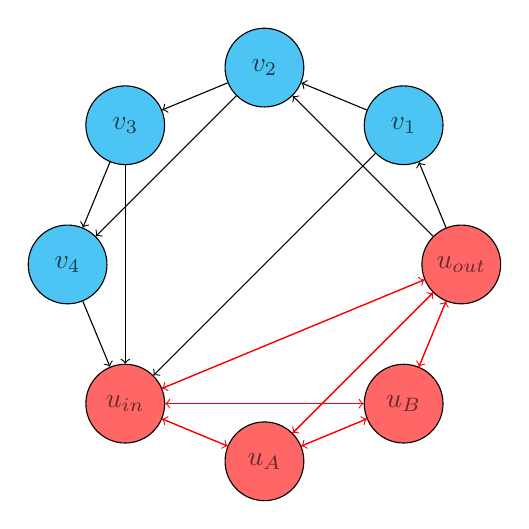
\begin{tikzpicture}
    % Define coordinates for octagon
    \coordinate (center) at (0,0);
    \foreach \i in {1,...,8} {
        \coordinate (v\i) at ({45*\i}:2.5cm);
    }
    
    % Draw nodes
    \foreach \i in {1,...,4} {
        \node[shape=circle,draw=black,fill=cyan, fill opacity=0.7, minimum size = 1cm] (node\i) at (v\i) {$v_{\i}$};
    }
    \node[shape=circle,draw=black,fill=red, fill opacity=0.6, minimum size = 1cm] (node5) at (v5) {$u_{in}$};
    \node[shape=circle,draw=black,fill=red, fill opacity=0.6, minimum size = 1cm] (node6) at (v6) {$u_{A}$};
    \node[shape=circle,draw=black,fill=red, fill opacity=0.6, minimum size = 1cm] (node7) at (v7) {$u_{B}$};
    \node[shape=circle,draw=black,fill=red, fill opacity=0.6, minimum size = 1cm] (node8) at (v8) {$u_{out}$};

    % Draw edges
    \foreach \i [evaluate=\i as \nextnode using {int(mod(\i,4)+1)}] in {1,...,3} {
        \draw[->] (node\i) -- (node\nextnode);
    }
    \draw[->] (node1) -- (node5);
    \draw[->] (node2) -- (node4);
    \draw[->] (node3) -- (node5);
    \draw[->] (node4) -- (node5);
    \draw[->] (node8) -- (node1);
    \draw[->] (node8) -- (node2);
    % Draw every edge between the red nodes
    \draw[->, red] (node5) -- (node6);
    \draw[->, red] (node5) -- (node7);
    \draw[->, red] (node5) -- (node8);
    \draw[->, red] (node6) -- (node5);
    \draw[->, red] (node6) -- (node7);
    \draw[->, red] (node6) -- (node8);
    \draw[->, red] (node7) -- (node5);
    \draw[->, red] (node7) -- (node6);
    \draw[->, red] (node7) -- (node8);
    \draw[->, red] (node8) -- (node5);
    \draw[->, red] (node8) -- (node6);
    \draw[->, red] (node8) -- (node7);


\end{tikzpicture}

\end{document}